\section*{Abstract}
It is now widely accepted that the standard inferential toolkit used by the
scientific research community -- null-hypothesis significance testing (NHST) --
is not fit for purpose. Yet despite the threat posed to the scientific
enterprise, there is no agreement concerning alternative approaches for evidence
assessment. This lack of consensus reflects long-standing issues concerning
Bayesian methods, the principal alternative to NHST. We report on recent work
that builds on an approach to inference put forward over 70 years ago to address
the well-known ``Problem of Priors'' in Bayesian analysis, by reversing the
conventional prior-likelihood-posterior (``forward'') use of Bayes's Theorem.
Such Reverse-Bayes analysis allows priors to be deduced from the likelihood by
requiring that the posterior achieve a specified level of credibility. We
summarise the technical underpinning of this approach, and show how it opens up
new approaches to common inferential challenges, such as assessing the
credibility of scientific findings, setting them in appropriate context,
estimating the probability of successful replications, and extracting more
insight from NHST while reducing the risk of misinterpretation. We argue that
Reverse-Bayes methods have a key role to play in making Bayesian methods more
accessible and attractive for evidence assessment and research synthesis. As a
running example we consider a recently published meta-analysis from several
randomized controlled trials (RCTs) investigating the association between
corticosteroids and mortality in hospitalized patients with COVID-19.

\textbf{Key words}: Analysis of Credibility, Bayes factor, false positive risk,
meta-analysis, prior-data conflict, reverse-Bayes

\section{Introduction: the origin of Reverse-Bayes methods}\label{sec4:intro}
\begin{center}
\begin{minipage}{12cm}
  { { { ``We can make judgments of initial probabilities and infer final ones,
        or we can equally make judgments of final ones and infer initial ones by
        \emph{Bayes's theorem in reverse}.'' }}}
\end{minipage}
\end{center}
\begin{flushright}
   \citet[p. 29]{Good1983}
\end{flushright}

There is now a common consensus that the most widely-used methods of statistical
inference have led to a crisis in both the interpretation of research findings
and their replication \citep{Gelman2014, Wasserstein2016}. At the same time,
there is a lack of consensus on how to address the challenge
\citep{Matthews2017}, as highlighted by the plethora of alternative techniques
to null-hypothesis significance testing now being put forward, see for example
\citet{Wasserstein2019} and the references therein.
Especially striking is the relative dearth of alternatives based on Bayesian
concepts. Given their intuitive inferential basis and output
\citep{Wagenmakers2008, McElreath2018}, these would seem obvious candidates to
supplant the prevailing frequentist methodology. However, it is well-known that
the adoption of Bayesian methods continues to be hampered by several factors,
such as the belief that advanced computational tools are required to make
Bayesian statistics practical \citep{Green2015}. The most persistent of these is
that the full benefit of Bayesian methods demands specification of a prior level
of belief, even in the absence of any appropriate insight. This ``Problem of
Priors'' has cast a shadow over Bayesian methods since their emergence over 250
years ago \citep{McGrayne2011}, and has led to a variety of approaches, such as
prior elicitation, prior sensitivity analysis, and objective Bayesian
methodology; all have their supporters and critics.

One of the least well-known was suggested over 70 years ago \citep{Good1950} by
one of the best-known proponents of Bayesian methods during the
20\textsuperscript{th} century, I.J.~Good. It involves reversing the
conventional direction of Bayes's Theorem and determining the level of prior
belief required to reach a specified level of posterior belief, given the
evidence observed. This reversal of Bayes's Theorem allows the assessment of new
findings on the basis of whether the resulting prior is reasonable in the light
of existing knowledge. Whether a prior is plausible in the light of existing
knowledge can be assessed informally or more formally using techniques for
comparing priors with existing data as suggested by \citet{Box1980} and further
refined by \citet{Evans2006}, see also \citet{Nott2020, Nott2021} for related
approaches. Good stressed that despite the routine use of the adjectives
``prior'' and ``posterior'' in applications of Bayes's Theorem, the validity of
any resulting inference does not require a specific temporal ordering, as the
theorem is simply a constraint ensuring consistency with the axioms of
probability. While reversing Bayes's Theorem is still regarded as unacceptable
by some on the grounds it allows ``cheating'' in the sense of choosing priors to
achieve a desired posterior inference \citep[p. 143]{OHagan2004}, others point
out this is not an ineluctable consequence of the reversal \citep[pp.
78--79]{Cox2006}. As we shall show, recent technical advances further weaken
this criticism.



Good's belief in the value of Reverse-Bayes methods won support from E.T.~Jaynes
in his well-known treatise on probability. Explaining a specific manifestation
of the approach (to be discussed shortly) Jaynes remarked: ``We shall find it
helpful in many cases where our prior information seems at first too vague to
lead to any definite prior probabilities; it stimulates our thinking and tells
us how to assign them after all'' \citep[p. 126]{Jaynes2003}. Yet despite the
advocacy of two leading figures in the foundations of Bayesian methodology, the
potential of Reverse-Bayes methods has remained largely unexplored. Most
published work has focused on their use in putting new research claims in
context, with Reverse-Bayes methods being used to assess whether the prior
evidence needed to make a claim credible is consistent with existing insight
\citep{Carlin1996,Matthews2001a,Matthews2001b,Spiegelhalter2004,Greenland2006,Greenland2011,Held2013,Colquhoun2017,Colquhoun2019,Held2019a,Held2020,Pawel2020b,
  Best2021}.


The purpose of this paper is to highlight recent technical developments of
Good's basic idea which lead to inferential tools of practical value in the
analysis of summary measures as reported in meta-analysis. As a running example
we consider a recently published meta-analysis investigating the association
between corticosteroids and mortality in hospitalized patients with COVID-19.
Specifically, we show how Reverse-Bayes methods address the current concerns
about the interpretation of new findings and their replication. We begin by
illustrating the basics of the Reverse-Bayes approach for both hypothesis
testing and parameter estimation. This is followed by a discussion of
Reverse-Bayes methods for assessing effect estimates in Section
\ref{sec4:effects}. These allow the credibility of both new and existing research
findings reported in terms of NHST to be evaluated in the context of existing
knowledge. This enables researchers to go beyond the standard dichotomy of
statistical significance/non-significance, extracting further insight from their
findings. We then discuss the use of the Reverse-Bayes approach in the most
recalcitrant form of the Problem of Priors, involving the assessment of research
findings which are unprecedented and thus lacking any clear source of prior
support. We show how the concept of intrinsic credibility resolves this
challenge, and puts recent calls to tighten $p$-value thresholds on a principled
basis \citep{Benjamin2017}. In Section \ref{sec4:bfs} we describe Reverse-Bayes
methods with Bayes factors, the principled solution for Bayesian hypothesis
testing. Finally, we describe in Section \ref{sec4:p.equals} Reverse-Bayes
approaches to interpretational issues that arise in conventional statistical
analysis based on $p$-values, and how they can be used to flag the risk of
inferential fallacies. We close with some extensions and final conclusions.



\subsection{Reverse-Bayes for hypothesis testing}
The subjectivity involved in the specification of prior distributions is often
seen as a weak point of Bayesian inference. The Reverse-Bayes approach can help
to resolve this issue both in hypothesis testing and parameter estimation, we
will start with the former.

Consider a null hypothesis $H_0$ with prior probability $\pi=\P(H_0)$, so
$\P(H_1) =1-\pi$ is the prior probability of the alternative hypothesis $H_1$.
Computation of the posterior probability of $H_1$ is routine with Bayes'
theorem:
\begin{equation*}
  \Pr(H_{1} \given \data) = \frac{\Pr(\data \given H_{1}) \Pr(H_{1})}{\Pr(\data \given H_{0}) \Pr(H_{0}) +
    \Pr(\data \given H_{1}) \Pr(H_{1})}.
\end{equation*}
Bayes' theorem can be written in more compact form as
\begin{equation}\label{eq4:eq0}
  \frac{\Pr(H_{1} \given \data)}{\Pr(H_{0} \given \data)} =
  \frac{\Pr(\data \given H_{1})}{\Pr(\data \given H_{0})} \,  \frac{\Pr(H_{1})}{\Pr(H_{0})},
\end{equation}
\ie{} the posterior odds are the likelihood ratio times the prior odds. The
standard 'forward-Bayes' approach thus fixes the prior odds (or one of the
underlying probabilities), determines the likelihood ratio for the available
data, and takes the product to compute the posterior odds. Of course, the latter
can be easily back-transformed to the posterior probability
$\Pr(H_{1} \given \data)$, if required. The Problem of Priors is now apparent:
in order for us to update the odds in favour of $H_1$, we must first specify the
prior odds. This can be problematic in situations where, for example, the
evidence on which to base the prior odds is controversial or even non-existent.

However, as Good emphasised it is entirely justifiable to ``flip'' Bayes's
theorem around, allowing us to ask the question: Which prior, when combined with
the data, leads to our specified posterior?
\begin{equation}\label{eq4:eq1}
  \frac{\Pr(H_{1})}{\Pr(H_{0})} = \left. \frac{\Pr(H_{1} \given \data)}{\Pr(H_{0} \given \data)} \, \Big/
\,   \frac{\Pr(\data \given H_{1})}{\Pr(\data \given H_{0})} \right. .
\end{equation}

For illustration we re-visit an example put forward by \citet[p. 35]{Good1950},
perhaps the first published Reverse-Bayes calculation. It centres on a question
for which the setting of an initial prior is especially problematic: does an
experiment provide convincing evidence for the existence of extra-sensory
perception (ESP)? The substantive hypothesis $H_{1}$ is that ESP exists, so that
$H_{0}$ asserts it does not exist. Imagine an experiment in which a person has
to make $n$ consecutive guesses of random digits (between 0 and 9) and all are
correct, as the ESP hypothesis $H_{1}$ would predict. The likelihood ratio is
therefore
\begin{equation}\label{eq4:ESPlik}
   \frac{\Pr(\data \given H_{1})}{\Pr(\data \given H_{0})} = \frac{1}{(1/10)^n} = 10^n .
\end{equation}
It is unlikely that sceptics and advocates of the existence of ESP would ever
agree on what constitutes reasonable priors from which to start a standard
Bayesian analysis of the evidence. However, Good argued that Reverse-Bayes
offers a way forward by using it to set bounds on the prior probabilities for
$H_{1}$ and $H_{0}$. This is achieved via the outcome of a thought (Gedanken)
experiment capable of demonstrating $H_{1}$ is more likely than $H_{0}$, that
is, of leading to posterior probabilities such that
$\Pr(H_1 \given \data) > \Pr(H_0 \given \data)$. Using this approach, which Good
termed the \emph{Device of Imaginary Results}, we see that if the ESP experiment
produced $n=20$ correct consecutive guesses, \eqref{eq4:eq1} combined with
\eqref{eq4:ESPlik} implies that ESP may be deemed more likely than not to exist
by anyone whose priors satisfy ${\Pr(H_{1})}/{\Pr(H_{0})} > 10^{-20}$. In
contrast, if only $n = 3$ correct guesses emerged, then the existence of ESP
could be rejected by anyone whose priors satisfy
${\Pr(H_{1})}/{\Pr(H_{0})} < 10^{-3}$. Using Bayes's Theorem in reverse has thus
led to a quantitative statement of the prior beliefs that either advocates or
sceptics of ESP must be able to justify in the face of results from a real
experiment. The practical value of Good's approach was noted by Jaynes in his
treatise: ``[I]n the present state of development of probability theory, the
device of imaginary results is usable and useful in a very wide variety of
situations, where we might not at first think it applicable''
\citep[p. 125--126]{Jaynes2003}.

It is straightforward to extend \eqref{eq4:eq0} and \eqref{eq4:eq1} to hypotheses
that involve unknown parameters $\theta$. The likelihood ratio
$\Pr(\data \given H_{1})/\Pr(\data \given H_{0})$ is then called a Bayes factor
\citep{Jeffreys1961, Kass1995} where
\begin{equation*}
  \Pr(\data \given H_{i}) = \int \Pr(\data \given \theta, H_{i})\,
  \p(\theta \given H_{i}) \,\mathrm{d} \theta
\end{equation*}
is the marginal likelihood under hypothesis $H_i$, $i=0,1$, obtained be
integration of the ordinary likelihood with respect to the prior distribution
$\p(\theta \given H_i)$. We will apply the Reverse-Bayes approach to Bayes
factors in Section \ref{sec4:bfs} and \ref{sec4:p.equals}.


\subsection{Reverse-Bayes for parameter estimation}
We can also apply the Reverse-Bayes idea to continuous prior and posterior
distributions of a parameter of interest $\theta$. Reversing Bayes' theorem
\begin{equation*}
  \p(\theta \given \data) = \frac{\p(\data \given \theta) \p(\theta)}{\p(\data)}
\end{equation*}
then leads to
\begin{equation}
  \p(\theta) = \p(\data) \, \frac{\p(\theta \given \data)}{\p(\data \given \theta)}.
\label{eq4:revBayesDensity}
\end{equation}
So the prior is proportional to the posterior divided by the likelihood with
proportionality constant $\p(\data)$.

Consider Bayesian inference for the mean $\theta$ of a univariate normal
distribution, assuming the variance $\sigma^2$ is known. Let $x$ denote the
observed value from that $\Nor(\theta, \sigma^2)$ distribution and suppose the
prior for $\theta$ (and hence also the posterior) is conjugate normal. Each of
them is determined by two parameters, usually the mean and the variance, but two
distinct quantiles would also work. If we fix both parameters of the posterior,
then the prior in \eqref{eq4:revBayesDensity} is -- under a certain regularity
condition -- uniquely determined. For ease of presentation we work with the
observational precision $\kappa=1/\sigma^2$ and denote the prior and posterior
precision by $\delta$ and $\delta'$, respectively. Finally let $\mu$ and $\mu'$
denote the prior and posterior mean, respectively.

Forward-Bayesian updating tells us how to compute the posterior precision and
mean:
\begin{align}
\label{eq4:posterior-precision}
\delta' &= \delta + \kappa, \\
\mu' &= \frac{\mu \delta + x \kappa}{\delta'}.\label{eq4:posterior-mean}
\end{align}
For example, fixed-effect (FE) meta-analysis is based on iteratively applying
\eqref{eq4:posterior-precision} and \eqref{eq4:posterior-mean} to the summary
effect estimate $x_i$ with standard error $\sigma_i$ from the $i$-th study,
$i=1,\ldots,n$, starting with an initial precision of zero. Reverse-Bayes simply
inverts these equations, which leads to the following:
\begin{align}
\label{eq4:prior-precision}
\delta &= \delta' - \kappa,  \\
\mu &= \frac{\mu'\delta' - x \kappa}{\delta}, \label{eq4:prior-mean}
\end{align}
provided $\delta' > \kappa$, \ie{} the posterior precision must be larger than the
observational precision.

We will illustrate the application of \eqref{eq4:prior-precision} and
\eqref{eq4:prior-mean} as well as the methodology in the rest of this paper
using a recent meta-analysis combining information from $n=7$ randomized
controlled trials investigating the association between corticosteroids and
mortality in hospitalized patients with COVID-19 \citep{REACT2020}; its results
are reproduced in Figure \ref{fig4:covid19-meta} (here and henceforth, odds
ratios (ORs) are expressed as log odds ratios to transform the range from
$(0, \infty)$ to $(-\infty, +\infty)$, consistent with the assumption of
normality). Let $x_i = \hat \theta_i$ denote the maximum likelihood estimate
(MLE) of the log odds ratio $\theta$ in the $i$-th study with standard error
$\sigma_i$. The meta-analytic odds ratio estimate under the fixed-effect model
(the pre-specified primary analysis) is \mbox{$\widehat{\text{OR}} = 0.66$ [95\%
  CI $0.53$ to $0.82$]}, respectively \mbox{$\hat \theta = -0.42$ [95\% CI
  $-0.63$ to $-0.20$]} for the log odds ratio $\theta$, indicating evidence for
lower mortality of patients treated with corticosteroids compared to patients
receiving usual care or placebo. The pooled effect estimate $\hat \theta$
represents a posterior mean $\mu'$ with posterior precision $\delta'=83.8$.


\begin{figure}[!htb]
\begin{knitrout}
\definecolor{shadecolor}{rgb}{0.969, 0.969, 0.969}\color{fgcolor}
{\centering 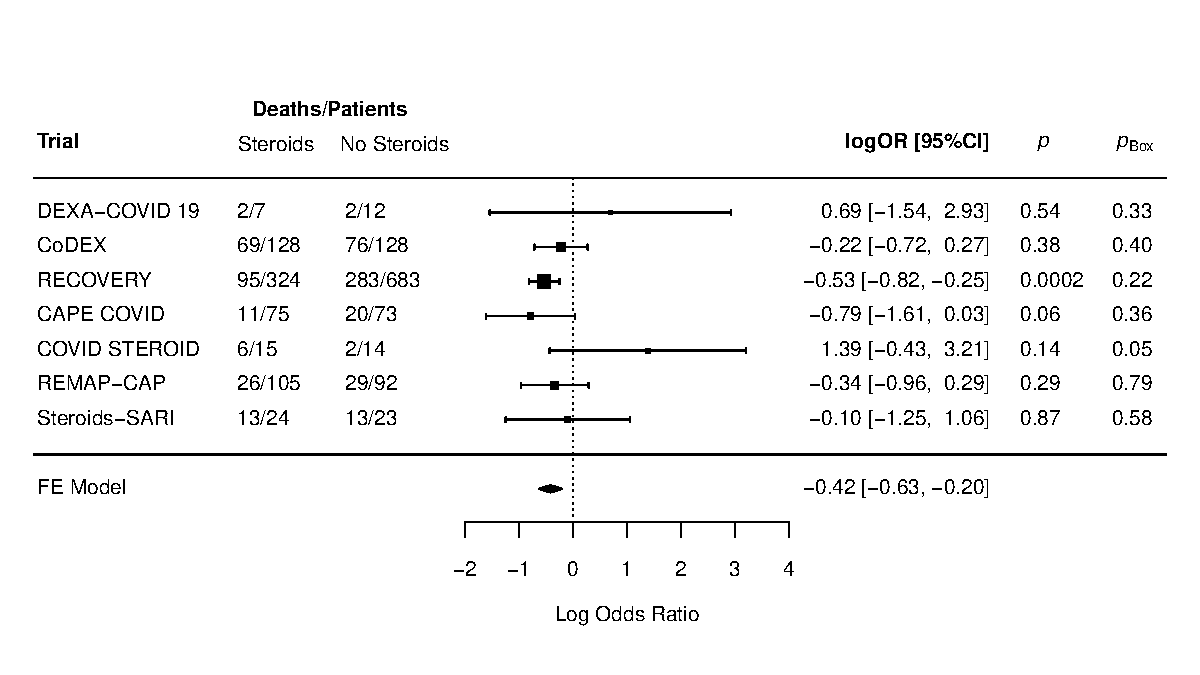
\includegraphics[width=\maxwidth]{images/paper4/forest-plot-covid19-1}
}
\end{knitrout}
\caption{Forest plot of fixed-effect meta-analysis of $7$ randomized controlled
  trials investigating association between corticosteroids and mortality in
  hospitalized patients with COVID-19 \citep{REACT2020}. Shown are number of
  deaths among total number of patients for treatment/control group, log odds
  ratio effect estimates with 95\% confidence interval, two-sided
  \textit{p}-values $p$, and prior-predictive tail probabilities
  $p_{\text{Box}}$ with a meta-analytic estimate based on the remaining studies
  serving as the prior.}
\label{fig4:covid19-meta}
\end{figure}



With a meta-analysis such as this, it is of interest to quantify potential
conflict among the effect estimates from the different studies. To do this, we
follow \citet{Presanis2013} and compute a prior-predictive tail probability
\citep{Box1980, Evans2006} for each study-specific estimate $\hat \theta_i$,
with a meta-analytic estimate based on the remaining studies serving as the
prior. As discussed above, fixed-effect meta-analysis is standard
forward-Bayesian updating for normally distributed effect estimates with an
initial flat prior. Hence, instead of fitting a reduced meta-analysis for each
study, we can simply use the the Reverse-Bayes equations
\eqref{eq4:prior-precision} and \eqref{eq4:prior-mean} together with the overall
estimate to compute the parameters of the prior in the absence of the $i$-th
study (denoted by the index $-i$):
\begin{eqnarray*}
\delta_{-i} & = & \delta' - 1/\sigma_i^2, \\
\mu_{-i} & = & \frac{ \mu' \delta' - \hat \theta_i / \sigma_i^2}{\delta_{-i}}.
\end{eqnarray*}
For example, through omitting the RECOVERY trial result $\hat{\theta}_i = -0.53$
with standard error ${\sigma}_i = 0.145$ we obtain $\delta_{-i} = 36.1$ and
$\mu_{-i} = -0.26$. A prior predictive tail probability using the approach from
\citet{Box1980} is then obtained by computing
$p_{\text{Box}} = \P(\chi^2_1 \geq t^2_{\text{Box}})$ with
$$
t_{\text{Box}} = \frac{\hat \theta_i - \mu_{-i}}{\sqrt{\sigma_i^2 + 1/\delta_{-i}}} =-1.24.$$
This leads to $p_{\text{Box}} = 0.22$ for the RECOVERY trial, indicating very
little prior-data conflict. The tail probabilities for the other studies are
even larger, with the exception of the COVID STEROID trial
($p_{\text{Box}}=0.05$), see Figure \ref{fig4:covid19-meta}. The lack of strong
conflict can be seen as an informal justification of the assumptions of the
underlying fixed-effect meta-analysis \citep{Presanis2013,Ferkingstad2017}. A
related method in network meta-analysis is to assess consistency via
``node-splitting'' \citep{Dias2010}. Reverse-Bayes methods may also be useful
for conflict assessment in more general evidence synthesis methods where
multiple distinct sources of data are combined \citep{Goodie2019,Cunen2021}, but
this may require more advanced numerical techniques.




Instead of determining the prior completely based on the posterior, one may also
want to fix one parameter of the posterior and one parameter of the prior. This
is of particular interest in order to challenge ``significant'' or
``non-significant'' findings through the Analysis of Credibility, as we will see
in the following section.


\section{Reverse-Bayes methods for the assessment of effect estimates}\label{sec4:effects}
A more general question amenable to Reverse-Bayes methods is the assessment of
effect estimates and their statistical significance or non-significance. This
issue has recently attracted intense interest following the public statement of
the American Statistical Association about the misuse and misinterpretation of
the NHST concepts of statistical significance and non-significance
\citep{Wasserstein2016}. First investigated 20 years ago by
\citet{Matthews2001a, Matthews2001b}, Reverse-Bayes methods for assessing both
statistically significant and non-significant findings have been termed the
Analysis of Credibility, or in short AnCred \citep{Matthews2018}, whose
principles and practice we now briefly review.

\subsection{The Analysis of Credibility}
\label{sec4:AnCred}
Suppose the study gives rise to a conventional confidence interval for the
unknown effect size $\theta$ at level $1 - \alpha$ with lower limit $L$ and
upper limit $U$. Assume that $L$ and $U$ are symmetric around the point estimate
$\hat \theta$ (assumed to be normally distributed with standard error $\sigma$).
AnCred then takes this likelihood and uses a Reverse-Bayes approach to deduce
the prior required in order to generate credible evidence for the existence of
an effect, in the form of a posterior that excludes no effect. As such, AnCred
allows evidence deemed \emph{statistically significant}/\emph{non-significant}
in the NHST framework to be assessed for its \emph{credibility} in the Bayesian
framework. As the latter conditions on the data rather than the null hypothesis,
it is inferentially directly relevant to researchers. After a suitable
transformation AnCred can be applied to a large number of commonly used effect
measures such as differences in means, odds ratios, relative risks and
correlations. We refer to the literature of meta-analysis for details about
conversion among effect size scales, \eg{} \citet[chapter 11.6]{Cooper2019}. The
inversion of Bayes's Theorem needed to assess credibility requires the form and
location of the prior distribution to be specified. This in turn depends on
whether the claim being assessed is statistically significant or
non-significant; we consider each below.


\subsubsection{Challenging statistically significant findings}
\label{sec4:significantFindings}

A statistically significant finding at level $\alpha$ is characterized by both
$L$ and $U$ being either positive or negative. Equivalently
$z^2 > z_{\alpha/2}^2$ is required where $z=\hat \theta/\sigma$ denotes the
corresponding test statistic and $z_{\alpha/2}$ the $(1-\alpha/2)$-quantile of
the standard normal distribution.

For significant findings, the idea is to ask how sceptical we would have to be
not to find the apparent effect estimate convincing. To this end, a
\emph{sceptical prior} is derived such that the corresponding posterior credible
interval just includes zero, the value of no effect. This critical prior
interval can then be compared with internal or external evidence to assess if
the finding is credible or not, despite being ``statistically significant''.


More specifically, a Reverse-Bayes approach is applied to significant confidence
intervals (at level $\alpha$) based on a normally distributed effect estimate.
The sceptical prior is a mean-zero normal distribution with variance
$\tau^2 = g \cdot \sigma^2$, so the only free parameter is the relative prior
variance $g = \tau^2/\sigma^2$. The posterior is hence also normal and either
its lower $\alpha/2$-quantile (for positive $\hat{\theta}$) or upper
$1 - \alpha/2$-quantile (for negative $\hat{\theta}$) is fixed to zero, so just
represents ``non-credible''. The sufficiently sceptical prior then has relative
variance
\begin{align}
  \label{eq4:sspv}
  g &=
      \begin{cases}
        \dfrac{1}{z^2/z_{\alpha/2}^2 - 1}
        & ~~ \text{if} ~
        {z^2} > {z_{\alpha/2}^2} \\
        \text{undefined} & ~~ \text{else}
      \end{cases}
\end{align}
see the Appendix in \citet{Held2019a} for a derivation. The corresponding
\emph{scepticism limit} \citep{Matthews2018}, the upper bound of the
equal-tailed sceptical prior credible interval at level $1-\alpha$, is
\begin{equation}
  \label{eq4:S}
  \SL = \frac{(U-L)^2}{4 \sqrt{UL}},
\end{equation}
which holds for any value of $\alpha$ provided the effect is significant at that
level.


The left plot in Figure \ref{fig4:anCredEx} illustrates the AnCred procedure for
the finding from the RECOVERY trial, the only statistically significant result
(at the conventional $\alpha=0.05$ level) shown in Figure
\ref{fig4:covid19-meta}. The trial found a decrease in COVID-19 mortality for
patients treated with corticosteroids compared to usual care or placebo
($\hat{\theta} = -0.53$ [95\% CI $-0.82$ to $-0.25$]. The sufficiently sceptical
prior has relative variance $g = 0.39$, so the sufficiently sceptical prior
variance needs to be roughly 2.5 times smaller than the variance of the estimate
to make the result non-credible. The scepticism limit on the log odds ratio
scale turns out to be $\SL=0.18$, which corresponds to a critical prior interval
with limits 0.84 and 1.19 on the odds ratio scale. Thus sceptics may still
reject the RECOVERY trial finding as lacking credibility despite its statistical
significance if external evidence suggests mortality reductions (in terms of
odds) are unlikely to exceed $1 - 0.84 \approx 16 \%$.


It is also possible to apply the approach to the meta-analytic log odds ratio
estimate \mbox{$\hat \theta = -0.42$ [95\% CI $-0.63$ to $-0.20$]} from all 7
studies combined. Then $\SL= 0.13$, so the meta-analytic estimate can be
considered as non-credible if external evidence suggests that mortality
reductions are unlikely to exceed $1-\exp(-\SL)=1 - 0.88 \approx 12 \%$. This
illustrates that the meta-analytic estimate has gained credibility compared to
the result from the \mbox{RECOVERY} study alone, despite the reduction in the
effect estimate ($\widehat{\text{OR}} = \exp(\hat \theta) = 0.66$ vs.~0.59 in
the RECOVERY study).

\subsubsection{Challenging statistically non-significant findings}
\label{sec4:nonSigAnCred}
It is also possible to challenge ``non-significant'' findings (\ie{} those for
which the CI now includes zero, so $z^2 < z_{\alpha/2}^2$) using a prior that
pushes the posterior towards being credible in the Bayesian sense, with
posterior credible interval no longer including zero, corresponding to no
effect.

\citet{Matthews2018} proposed the ``advocacy prior'' for this purpose, a normal
prior with positive mean $\mu$ and variance $\tau^2$ chosen such that the
$\alpha/2$-quantile is fixed to zero (for positive effect estimates
$\hat \theta > 0$). He showed that the ``advocacy limit'' AL, the
$(1-\alpha/2)$-quantile of the advocacy prior is
\begin{equation}\label{eq4:AL}
  \mbox{AL} = - \frac{U+L}{2 \, U L} (U-L)^2
\end{equation}
to reach credibility of the corresponding posterior at level $\alpha$. We show
in Appendix \ref{app:app1} that the corresponding relative prior mean
$f = \mu / \hat \theta$ is
\begin{align}
\label{eq4:mu}
  f &=
  \begin{cases}
    \dfrac{2}{1 - z^2/z_{\alpha/2}^2}
    & ~~ \text{if} ~
    {z^2} < {z_{\alpha/2}^2} \\
    \text{undefined} & ~~ \text{else. }
\end{cases}
\end{align}

There are two important properties of the advocacy prior. First, the coefficient
of variation CV is
$$\mbox{CV} = \tau/\mu = z_{\alpha/2}^{-1}.$$
The advocacy prior $\theta \sim \Nor(\mu, \tau^2=\mu^2 \, \mbox{CV}^2)$ is hence
characterized by a fixed coefficient of variation, so this prior has equal
evidential weight (quantified in terms of $\mu/\tau=z_{\alpha/2}$) as data which
are ``just significant'' at level $\alpha$. Second, the advocacy limit AL
defines the family of normal priors capable of rendering a ``non-significant''
finding credible at the same level. Such priors are summarized by the credible
interval ($L_o, U_o$) where $L_o \geq 0$, $U_o \leq \mbox{AL}$. Thus when
confronted with a ``non-significant'' result -- often, and wrongly, interpreted
as indicating no effect -- advocates of the existence of an effect may still
claim the existence of the effect is credible to the same level if there exists
prior evidence or insight compatible with the credible interval ($L_o, U_o$). If
the evidence for an effect is strong (weak), the resulting advocacy prior will
be broad (narrow), giving advocates of an effect more (less) latitude to make
their case under terms of AnCred. Note that \eqref{eq4:AL} and \eqref{eq4:mu}
also hold for negative effect estimates, where we fix the
$(1-\alpha/2)$-quantile of the advocacy prior to zero and define the advocacy
limit AL as the $\alpha/2$-quantile of the advocacy prior.

\begin{figure}[!htb]
\begin{knitrout}
\definecolor{shadecolor}{rgb}{0.969, 0.969, 0.969}\color{fgcolor}
{\centering 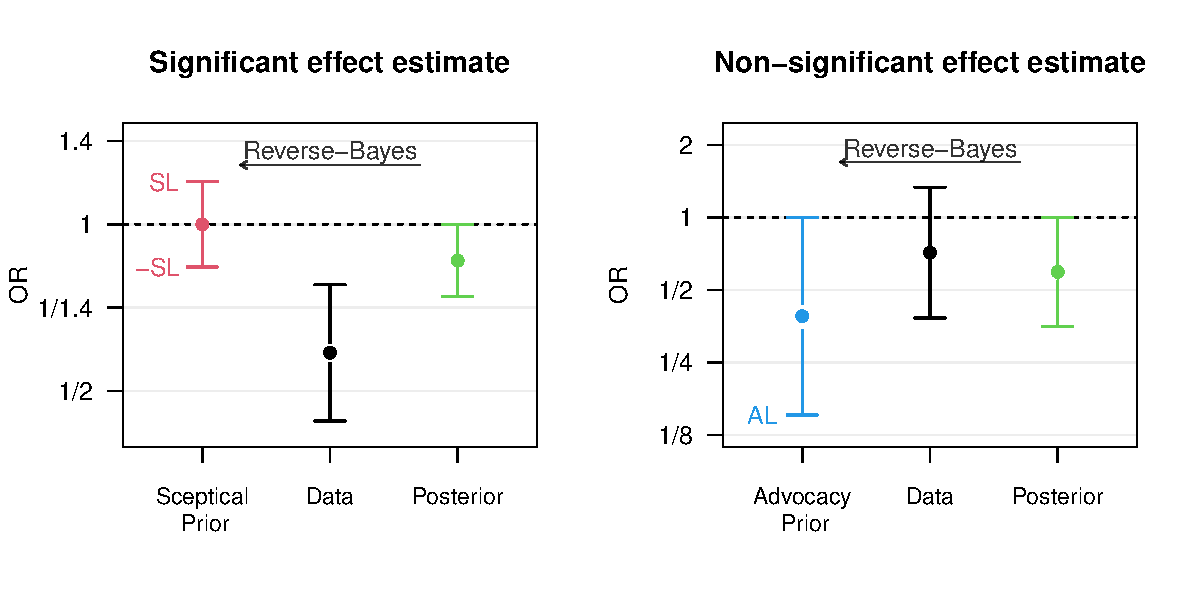
\includegraphics[width=\maxwidth]{images/paper4/AnCred-examples-plot-1}
}
\end{knitrout}
\caption{Two examples of the Analysis of Credibility. Shown are point estimates
  within 95\% confidence/credible intervals. The left plot illustrates how a
  sceptical prior is used to challenge the significant finding from the RECOVERY
  trial \citep{RECOVERY2020}. The right plot illustrates how an advocacy prior
  is used to challenge a non-significant finding from the \mbox{REMAP-CAP} trial
  \citep{REMAPCAP2020}. In both scenarios the posterior is fixed to be just
  non-credible/credible.}
\label{fig4:anCredEx}
\end{figure}

For illustration we consider the data from the REMAP-CAP trial that supported
the RECOVERY trial finding of decreased COVID-19 mortality from corticosteroid
use. However, this trial involved far fewer patients, and despite the point
estimate showing efficacy, the relatively large uncertainty rendered the overall
finding non-significant at the 5\% level (\mbox{$\hat{\theta} = -0.34$ [95\% CI
  $-0.96$ to $0.29$]}). Such an outcome is frequently (and wrongly) taken to
imply no effect. The use of AnCred leads to a more nuanced conclusion. The
advocacy limit AL on the log odds ratio scale for REMAP-CAP is $-1.89$, \ie{}
$0.15$ on the odds ratio scale, see also the right plot in Figure
\ref{fig4:anCredEx}. Thus advocates of the effectiveness of corticosteroids can
regard the trial as providing credible evidence of effectiveness despite its
non-significance if external evidence supports mortality reductions (in terms of
odds) in the range 0\% to 85\%. So broad an advocacy range reflects the fact
that this relatively small trial provides only modest evidential weight, and
thus little constraint on prior beliefs about the effectiveness of
corticosteroids.

Another way to push non-significant findings towards credibility is to use a
prior based on data from another study or a different subgroup. For example,
\citet{Best2021} consider results from the MENSA trial \citep{MENSA2014} on the
efficacy of Mepolizumab against placebo in 551 adult and 25 adolescent patients
with severe asthma. The treatment effect was estimated to be positive in both
subgroups but lacked significance among adolescents. Best et al. combine the
data in the adolescent subgroup with a mixture prior based on a weak and an
informative component. The weak component is a minimally informative normal
prior with mean zero and large variance. The variance is chosen such that the
information content of the prior is equivalent to that provided by a single
subject or event \citep[\emph{unit-information prior},][]{Kass1995b}. The other
component is an informative prior based on the (significant) results from the
adolescent subgroup. A Reverse-Bayes approach is used to determine how much
prior weight one needs to assign to the informative component to obtain a
credible posterior result with a 95\% highest posterior credible interval no
longer including zero. In the MENSA trial the required prior weight on the
informative component was 0.7 (and thus 0.3 on the weak prior component) to
achieve a credible result \citep{Best2021}. This illustrates that a considerable
amount of ``Bayesian borrowing'' is required to extrapolate the results from
adults to adolescents.

\begin{figure}[!htb]
\begin{knitrout}
  \definecolor{shadecolor}{rgb}{0.969, 0.969, 0.969}\color{fgcolor}
{\centering 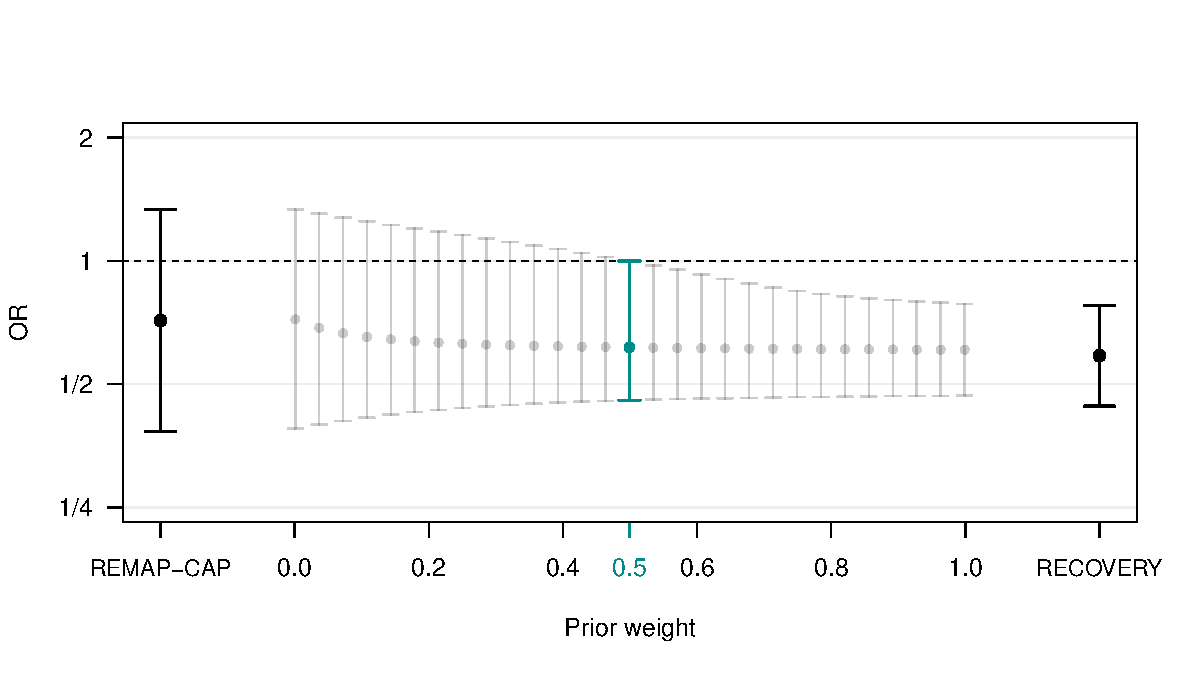
\includegraphics[width=\maxwidth]{images/paper4/advocacy-borrowing-1}
}
\end{knitrout}
\caption{Illustration of the Reverse-Bayes borrowing method. The data from the
  (non-significant) REMAP-CAP trial are combined with a mixture prior consisting
  of the (significant) RECOVERY trial data and a unit-information prior (both
  estimates shown with 95\% confidence interval). The resulting posterior
  medians with equal-tailed 95\% credible intervals are shown for a range of
  mixing weights. The Reverse-Bayes mixing weight $w = 0.5$ leads to the
  highlighted posterior with upper credible interval limit fixed at one.}
\label{fig4:borrowing}
\end{figure}
In the meta-analytic setting we may ask a similar question: Suppose we want to
combine the REMAP-CAP study results with a fraction of the RECOVERY trial data,
how much weight do we need to assign to the RECOVERY trial to make the REMAP-CAP
study credible? The unit-information prior for a logOR has variance
$\tau^{2} = 4$ \citep[section 2.4.1]{Spiegelhalter2004}, so the mixture prior is
\begin{align*}
  \theta \sim w \cdot \Nor\left(0, \tau^{2} = 4\right) + (1 - w) \cdot
  \Nor\left( \hat{\theta}_{\scriptscriptstyle \text{REC}},
  \sigma^{2}_{\scriptscriptstyle \text{REC}}\right)
\end{align*}
with $w$ the mixing weight and point estimate
$\hat{\theta}_{\scriptscriptstyle \text{REC}}$ and squared standard error
$\sigma^{2}_{\scriptscriptstyle \text{REC}}$ of the RECOVERY trial,
respectively. The resulting posterior is again a mixture of two normals with the
posterior mean and variance of each component being the usual ones obtained from
conjugate Bayesian updating, while the weights are proportional to the marginal
likelihood of the data under each component \citep[section 3.5]{Best2021}.

Figure~\ref{fig4:borrowing} shows posterior medians with 95\% equal-tailed
credible intervals for a range of mixing weights. We see that a weight of at
least $w = 0.5$ is required to render the resulting posterior credible.
Advocates of corticosteroids thus need to be able to justify such levels of
prior beliefs, in order to conclude efficacy of corticosteroids also in the
REMAP-CAP trial.




\subsubsection{Assessing credibility via equivalent prior study sizes}
\label{sec4:prior-data-translation}
Reverse-Bayes credibility assessments can also be formulated in terms of the
size and content of a prior study capable of challenging a claim of statistical
significance/non-significance. This approach puts the weight of prior evidence
in the context of the observed data, expressed as participant numbers.
\citet{Greenland2006} demonstrated the value of this approach in assessing the
credibility of statistically significant findings from large observational
studies in epidemiology. The same concept can, however, be extended to the
assessment of both significant and non-significant outcomes more widely, such as
small randomized controlled trials. For any study generating binary data in the
form of event/non-event counts under two different conditions, the comparative
effect measure can be expressed as a log-odds ratio with variance (squared
standard error)
\begin{equation}
  \label{eq4:SElogOR}
%% \tau^{2} =
1/m_1 + 1/n_1 + 1/m_2 + 1/n_2.
\end{equation}
where $m_i$ and $n_i$ are the numbers of events and non-events, respectively, in
study arm $i=1,2$. This provides the link between the Reverse-Bayes prior
distribution and the corresponding numbers of prior study participants. Using
the simplifying assumptions of equal numbers of events $m = m_{1} = m_{2}$ and
large numbers of non-events $n_{1}$ and $n_2$ in each arm ($n_i > 100 \, m_i$,
say), the variance \eqref{eq4:SElogOR} reduces to $2/m$. The Reverse-Bayes
sceptical prior defined in Section \ref{sec4:significantFindings} has variance
$\tau^{2} = \SL^2/z_{\alpha/2}^{2}$, where $\SL$ is the sceptical limit.
Equating the two implies that such a prior is equivalent to a (large)
hypothetical study with $$m = 2/\tau^{2} = 2 \, z_{\alpha/2}^2/\SL^2$$ events in
both arms. The more compelling the data -- that is, the smaller the value of
$\SL$ -- the larger the number of events $m$ required in both arms of the
hypothetical large prior study to render the result non-credible at level
$\alpha$.

While the assumption of large studies can be appropriate with epidemiological
studies involving rare events, it can be harder to justify for RCTs.
Fortunately, the theory can be extended to encompass these and also the case of
non-significant findings with little additional complexity. In the case of the
sceptical prior, we simply require that the numbers of event $m$ and non-events
$n$ are the same in both arms to constrain the mean to zero; the variance
\eqref{eq4:SElogOR} then simplifies to $2/m + 2/n$. Adding the constraint that
the event rate of the sceptical prior $R= m /(m + n)$ matches that of the study
under assessment, we then find
\begin{eqnarray*}
  m = \frac{2}{\tau^{2}(1 - R)} & \mbox{ and }
  &n = \frac{m(1 - R)}{R}.
\end{eqnarray*}
For example, from Figure~\ref{fig4:covid19-meta} the RECOVERY trial has an
overall mortality rate \mbox{$R=(95 + 283)/(324 + 683) = 37.54\%$} and
$\SL = 0.178$ at the $\alpha = 5\%$ level $(z_{\alpha/2} = 1.96)$ corresponds to
$\tau^2=0.091^2$, so $m = 389$ and $n = 648$ (these are integer approximations
of exact computations), and thus a prior study capable of challenging the
credibility of the RECOVERY trial requires $1037$ patients and $389$ deaths in
each arm. At more than twice the size of the RECOVERY trial ($2074$ vs. $1007$)
patients and considerably more deaths in both arms, this level of sceptical
prior evidence highlights the robustness of the trial finding.


A similar approach determines the characteristics of the hypothetical prior
study needed to turn a ``negative'' non-significant finding into one that is
credible to a specific $\alpha$ level. The Reverse-Bayes advocacy prior from
\citet{Matthews2018} described in Section~\ref{sec4:nonSigAnCred} has a mean
\mbox{$\mu = \mbox{AL}/2$} and variance $\tau^{2} = \AL^2/(2z_{\alpha/2})^2$.
Under the large study assumption and equating the latter with
\eqref{eq4:SElogOR} as before, the corresponding number of events needed to be
observed in both arms of the hypothetical study is
$m = 2/\tau^{2} = 8 \, z_{\alpha/2}^2/\mbox{AL}^2$. To incorporate the non-zero
mean by which this prior represents advocacy, these $m$ events are taken to have
been observed among participants allocated to the two study arms in the ratio
$1 \colon K$ where \mbox{$K = \exp(\mu) = \exp(\AL/2)$}, the allocation being
such that it increases the relative evidential weight for the hypothesis
``negated'' by the non-significance.


As before, while the large study approximation may be justified in
epidemiological examples, this is less likely to be true for RCTs. In such
cases, we can adapt the approach used for sceptical priors, the size and
composition of the advocacy prior being found by setting the numbers of events
$m$ in each arm the same, but this time allowing for different numbers of
non-events in each arm via the allocation ratio $K$. The resulting variance is
then
\begin{align*}
  \tau^{2} = \frac{2}{m} + \frac{K + 1}{n}
\end{align*}
where $n$ is the number of non-events in the arm used to support the null
hypothesis (\eg{} the control arm in an RCT). With the control arm event rate
$R = m/(m + n)$ constrained to match that of the actual study, we find
\begin{eqnarray*}
  m = \frac{2 - R(1 - K)}{\tau^{2}(1 - R)} & \mbox{ and }
  &n = \frac{m(1 - R)}{R}.
\end{eqnarray*}

As an example, we return to the REMAP-CAP trial, whose findings were consistent
with a reduction of mortality but failed to reach statistical significance. As
noted above, its advocacy limit ($\AL = -1.89)$ implies this trial has
relatively little evidential weight, and gives considerable scope for prior
studies to make its outcome credible at the 95\% level. With
$K = \exp(\mu) = \exp(\AL/2) = 0.39$, $R = 29/92$ and $z_{\alpha/2} = 1.96$ we
find $m = 11$ and $n = 25$. Thus the hypothetical prior study comprises $11$
deaths from $11$ + $25$ = $36$ patients in the control arm and the same number
of deaths from $11 + (25/0.4) = 75$ patients in the treatment arm. At barely
half the total size of REMAP-CAP but a considerably more impressive mortality
reduction from $R = 29/92 = 32\%$ in the control arm to $11/75=15$\% in the
treatment arm (rather than $26/105=25$\% in REMAP-CAP), the nature of this
hypothetical prior study confirms the paucity of evidence in the original trial.



\subsubsection{The fail-safe \textit{N} method}
Another data representation of a sceptical prior forms the basis of the
well-known ``fail-safe $N$'' method, sometimes also called ``file-drawer
analysis''. This method, first introduced by \citet{Rosenthal1979} and later
refined by \citet{Rosenberg2005}, is commonly applied to the results from a
meta-analysis and answers the question: ``How many unpublished negative studies
do we need to make the meta-analytic effect estimate non-significant?'' A
relatively large $N$ of such unpublished studies suggests that the estimate is
robust to potential null-findings, for example due to publication bias.
Calculations are made under the assumption that the unpublished studies have an
average effect of zero and a precision equal to the average precision of the
published ones.

While the method does not identify nor adjust for publication bias, it provides
a quick way to assess how robust the meta-analytic effect estimate is. The
method is available in common software packages such as \texttt{metafor}
\citep{Viechtbauer2010} and its simplicity and intuitive appeal have made it
very popular among researchers.



AnCred and the fail-safe $N$ are both based on the idea to challenge effect
estimates such that they become ``non-significant/not credible'', and it is easy
to show that the methods are under some circumstances also technically
equivalent. To illustrate this, we consider again the meta-analysis on the
association between corticosteroids and COVID-19 mortality \citep{REACT2020}
which gave the pooled log odds ratio estimate $\hat \theta = -0.42$ with
standard error $\sigma = 0.11$, posterior precision $\delta'=83.8$ and test
statistic $z=\hat \theta/\sigma= -3.81$.


Using the \citet{Rosenberg2005} approach (as implemented in the \texttt{fsn()}
function from the \texttt{metafor} package) we find that at least $N = 20$
additional but unpublished non-significant findings are needed to make the
published meta-analysis effect non-significant. If instead, we challenge the
overall estimate with AnCred, we obtain the relative prior variance $g = 0.36$
using equation \eqref{eq4:sspv}, so $\tau^2 = 0.0043$. Taking into account the
average precision $\delta' / n = 11.98$ of the different effect estimates
estimates in the meta-analysis leads to ${N} = n/(\delta' \cdot \tau^2) = 19.5$
which is equivalent to the fail-safe $N$ result after rounding to the next
larger integer.


\subsection{Intrinsic credibility}
\label{sec4:IC}

The Problem of Priors is at its most challenging in the context of entirely
novel ``out of the blue'' effects for which no obviously relevant external
evidence exist. By their nature, such findings often attract considerable
interest both within and beyond the research community, making their reliability
of particular importance. Given the absence of external sources of evidence,
\citet{Matthews2018} proposed the concept of \emph{intrinsic
  credibility}. This requires that the evidential weight of an unprecedented
finding is sufficient to put it in conflict with the sceptical prior rendering
it non-credible. In the AnCred framework, this implies a finding possesses
intrinsic credibility at level $\alpha$ if the estimate $\hat{\theta}$ is
outside the corresponding sceptical prior interval $[-\SL, \SL]$ extracted using
Reverse-Bayes from the finding itself, \ie{} $\hat{\theta}^2 > \SL^2$ with $\SL$
given in \eqref{eq4:S}. Matthews showed this implies an unprecedented finding is
intrinsically credible at level $\alpha=0.05$ if its $p$-value does not exceed
0.013.

\citet{Held2019a} refined the concept by suggesting the use of a
prior-predictive check \citep{Box1980, Evans2006} to assess potential prior-data
conflict. With this approach the uncertainty of the estimate $\hat{\theta}$ is
also taken into account since it is based on the prior-predictive distribution,
in this case $\hat\theta \sim \Nor(0, \sigma^2 + \tau^2=\sigma^2 \, (1+g))$ with
$g$ as given in \eqref{eq4:sspv}. Intrinsic credibility is declared if the
(two-sided) tail-probability
\begin{equation*}
  p_{\text{Box}} = \P\left(\chi^2_1 \geq \hat \theta^2/(\sigma^2+\tau^2)\right) = \P\left(\chi^2_1 \geq z^2/(1+g)\right)
\end{equation*}
of $\hat{\theta}$ under the prior-predictive distribution is smaller than
$\alpha$. It turns out that the $p$-value associated with $\theta$ needs to be
at least as small as 0.0056 to obtain intrinsic credibility at level
$\alpha=0.05$, providing another principled argument for the recent proposition
to lower the \mbox{$p$-value} threshold for the claims of new discoveries to
0.005 \citep{Benjamin2017}. A simple check for intrinsic credibility is based on
the \emph{credibility ratio}, the ratio of the upper to the lower limit (or vice
versa) of a confidence interval for a significant effect size estimate. If the
credibility ratio is smaller than 5.8 then the result is intrinsically credible
\citep{Held2019a}. This holds for confidence intervals at all possible values of
$\alpha$, not just for the 0.05 standard. For example, in the RECOVERY study the
95\% confidence interval for the log-odds ratio ranges from $-0.82$ to $-0.25$,
so the credibility ratio is $-0.82/-0.25 = 3.27 < 5.8$ and the result is
intrinsically credible at the standard 5\% level.


\subsubsection*{Replication of effect direction}

Whether intrinsic credibility is assessed based on the prior or the
prior-predictive distribution, it depends on the level $\alpha$ in both cases.
To remove this dependence, \citet{Held2019a} proposed to consider the
smallest level at which intrinsic credibility can be established, defining the
$p$-value for intrinsic credibility
\begin{align}
  \label{eq4:pic}
  \pIC
  &= 2\left\{1 - \Phi\left(\frac{\abs{z}}{\sqrt{2}}\right)\right\},
\end{align}
see section 4 in \citet{Held2019a} for the derivation. Now
$z=\hat \theta/\sigma$, so compared to the standard $p$-value
$p=2\left\{1 - \Phi\left(\abs{z}\right)\right\}$, the $p$-value for intrinsic
credibility is based on twice the variance $\sigma^2$ of the estimate
$\hat{\theta}$. Although motivated from a different perspective, inference based
on intrinsic credibility thus mimics the \emph{doubling the variance rule}
advocated by \citet{Copas2005} as a simple means of adjusting for model
uncertainty.

Moreover, \citet{Held2019a} showed that $\pIC$ is connected to $\prep$ of
\citet{Killeen2005}, the probability that a replication will result in an effect
estimate $\hat{\theta}_r$ in the same direction as the observed effect estimate
$\hat{\theta}$, by $\prep = 1 - \pIC/2$. Hence, an intrinsically credible
estimate at a small level $\alpha$ will have high chance of replicating since
$\prep \geq 1 - \alpha/2$. Note that $\prep$ lies between 0.5 and 1 with the
extreme case $\prep=0.5$ if $\hat \theta=0$.

As an example, the $p$-value for intrinsic credibility for the RECOVERY trial
finding (with $p$-value $p=0.0002$) cited earlier is $\pIC = 0.01$ and thus the
probability of the replication effect going in the same direction (\ie{} reduced
mortality in this case) is $0.995$. In contrast, the finding from the smaller
REMAP-CAP trial (with $p=0.29$) leads to $\pIC = 0.46$, and the probability of
effect direction replication is hence only $0.77$.

\section{Reverse-Bayes methods with Bayes factors}
\label{sec4:bfs}
The AnCred procedure as described above uses posterior credible intervals as a
means of quantifying evidence. However, quantification of evidence with Bayes
factors is a more principled solution for hypothesis testing in the Bayesian
framework \citep{Jeffreys1961, Kass1995}. Bayes factors enable direct
probability statements about null and alternative hypothesis and they can also
quantify evidence \emph{for} the null hypothesis, both are impossible with
indirect measures of evidence such as $p$-values \citep{Held2018}.
Reverse-Bayes approaches combined with Bayes factor methodology was pioneered by
\citet{Carlin1996} but then remained unexplored until \citet{Pawel2020b}
proposed an extension of AnCred where Bayes factors are used as a means of
quantifying evidence. Rather than determining a prior such that a finding
becomes ``non-credible'' in terms of a posterior credible interval, this
approach determines a prior such that the finding becomes ``non-compelling'' in
terms of a Bayes factor. In the second step of the procedure, the plausibility
of this prior is quantified using external data from a replication study. Here,
we will illustrate the methodology using only an original study; we mention
extensions for replications in Section \ref{sec4:extensions}.

\subsection{Sceptical priors}\label{sec4:sceptical}

As before, $\hat \theta$ denotes the estimate of the unknown mean $\theta$ of a
$\Nor(\theta, \sigma^2)$ distribution with known variance $\sigma^2$. A standard
hypothesis test compares the null hypothesis $H_0\colon$ $\theta = 0$ to the
alternative $H_1\colon$ $\theta \neq 0$. Bayesian hypothesis testing requires
specification of a prior distribution of $\theta$ under $H_1$. A typical choice
is a local alternative, a unimodal symmetric prior distribution centred around
the null value \citep{Johnson2010}. We consider again the conjugate sceptical
prior $\theta \given H_1 \sim \Nor(0, \tau^2 = g \cdot \sigma^2)$ with relative
prior variance $g$ for this purpose. This leads to the Bayes factor comparing
$H_0$ to $H_1$ being
\begin{align}
  \label{eq4:bf01}
  \BF_{01} =
  \sqrt{1 + g} \cdot
  \exp\left\{-\frac{g}{1 + g} \cdot \frac{z^2}{2} \right\},
\end{align}
where $z=\hat \theta/\sigma$. Yet again, the amount of evidence which the data
provide against the null hypothesis depends on the prior parameter $g$; As $g$
becomes smaller ($g \downarrow 0$), the null hypothesis and the alternative will
become indistinguishable, so the data are equally likely under both
($\BF_{01} \to 1$). On the other hand, for increasingly diffuse priors
($g \to \infty$), the null hypothesis will always prevail
($\BF_{01} \to \infty$) due to the Jeffreys-Lindley paradox \citep{Robert2014}.
In between, the $\BF_{01}$ reaches a minimum at
$g = \max\left\{z^2 - 1, 0\right\}$ leading to
\begin{align}
  \text{minBF}_{01} =
  \begin{cases}
    \abs{z} \cdot \exp\left\{-z^2/2\right\} \cdot \sqrt{e}
    & \text{if} ~ \abs{z} > 1 \\
    1 & \text{else}
  \end{cases}
  \label{eq4:minBFnorm}
\end{align}
which is an instance of a \emph{minimum Bayes factor}, the smallest possible
Bayes factor within a class of alternative hypotheses, in this case zero-mean
normal alternatives \citep{Edwards1963, Berger1987, Sellke2001, Held2018}.

Reporting of minimum Bayes factors is one attempt of solving the Problem of
Priors in Bayesian inference. However, this bound may be rather small and the
corresponding prior unrealistic. In contrast, the Reverse-Bayes approach makes
the choice of the prior explicit by determining the relative prior variance
parameter $g$ such that the finding is no longer compelling, followed by
assessing the plausibility of this prior. To do so, one first fixes
$\BF_{01} = \gamma$, where $\gamma$ is a cut-off above which the result is no
longer convincing, for example $\gamma = 1/10$, the level for strong evidence
according to the classification from \citet{Jeffreys1961}. The sufficiently
sceptical relative prior variance is then given by
\begin{align}
\label{ggamma}
  g &=
  \begin{cases}
    -\dfrac{z^2}{q} - 1
    & ~~ \text{if} ~
    -\dfrac{z^2}{q} \geq 1 \\
    \text{undefined} & ~~ \text{else}
  \end{cases} \\
  \text{where} ~ q &=
  \mathrm{W} \left(-\frac{z^2}{\gamma^2} \cdot
  \exp\left\{-z^2\right\}\right)
  \nonumber
\end{align}
where $\mathrm{W}(\cdot)$ is the branch of the Lambert W function that satisfies
$\mathrm{W}(y) \leq -1$ for \mbox{$y \in [-e^{-1}, 0)$} \citep{Corless1996}, see
the Appendix in \citep{Pawel2020b} for a proof.

The sufficiently sceptical relative prior variance $g$ exists only for a cut-off
$\gamma$ if $\text{minBF}_{01} \leq \gamma$, similar to standard AnCred where it
exists only at level $\alpha$ if the original finding was significant at the
same level. In contrast to standard AnCred, however, if the sufficiently
sceptical relative prior variance $g$ exists, there are always two solutions, a
consequence of the Jeffreys-Lindley paradox: If $\BF_{01}$ decreases in $g$
below the chosen cut-off $\gamma$, after attaining its minimum it will
monotonically increase and intersect a second time with $\gamma$, admitting a
second solution for the sufficiently sceptical prior.


\begin{figure}[!htb]
\begin{knitrout}
\definecolor{shadecolor}{rgb}{0.969, 0.969, 0.969}\color{fgcolor}
{\centering 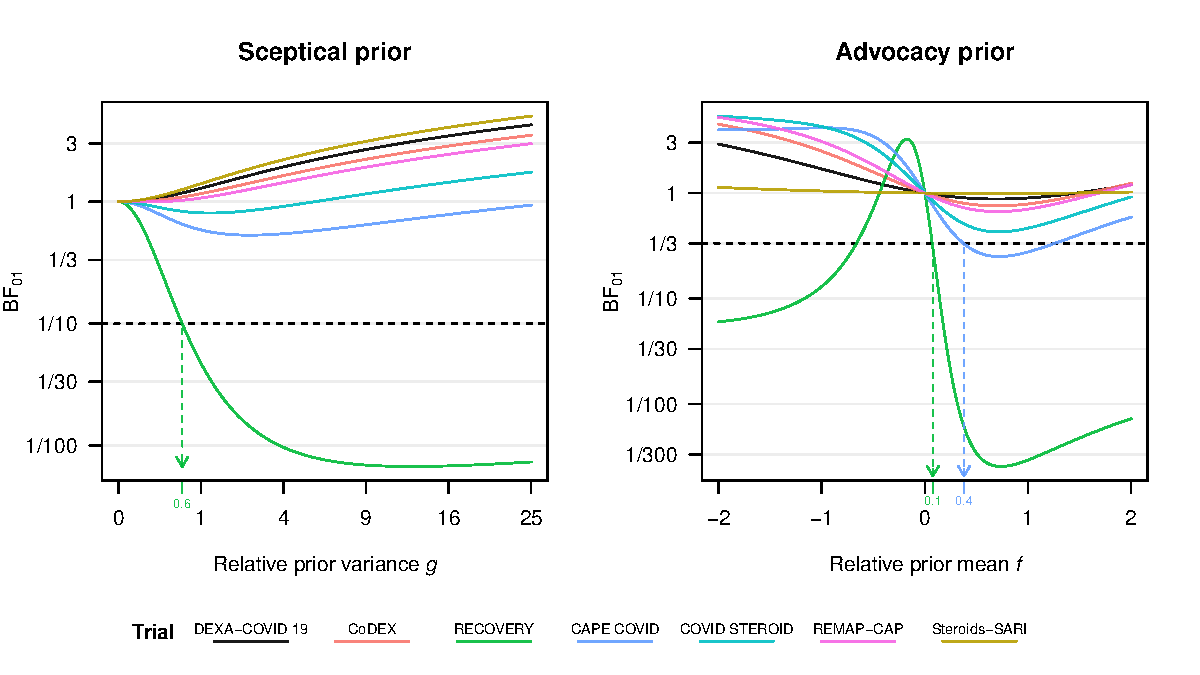
\includegraphics[width=\maxwidth]{images/paper4/AnCred-BF-examples-plot-1}
}
\end{knitrout}
\caption{Illustration of the AnCred with Bayes factors procedure using the
  findings from the meta-analysis on the association of COVID-19 mortality and
  corticosteroids. The left plot shows the Bayes factor $\BF_{01}$ as a function
  of the relative variance $g$ of the sceptical prior. The result from the
  RECOVERY trial is challenged with a sceptical prior such that
  $\BF_{01} = 1/10$, for the other trials such a prior does not exist. The right
  plot shows the Bayes factor $\BF_{01}$ as a function of the relative mean
  $f = \mu/\hat{\theta}$ of the advocacy prior where the coefficient of
  variation from the prior is fixed to
  \mbox{$\text{CV} = \tau/\mu = 1/z(\gamma=1/3) = 0.67$}, where $z(\gamma)$ is
  given in \eqref{eq4:zgamma}. The RECOVERY and the CAPE COVID findings are
  challenged such that $\BF_{01} = 1/3$, for the other trials such a prior does
  not exist.}
\label{fig4:bf}
\end{figure}

We now revisit the meta-analysis example considered earlier: The left plot in
Figure \ref{fig4:bf} shows the Bayes factor $\BF_{01}$ from~\eqref{eq4:bf01} as
a function of the relative prior variance $g$ for each finding included in the
meta-analysis. Most of them did not include a great number of participants and
thus provide little evidence against the null hypothesis for any value of the
relative prior variance $g$. In contrast, the finding from the RECOVERY trial
provides more compelling evidence and can be challenged up to
$\text{minBF}_{01} = 1/148.9$. For example, we see in Figure \ref{fig4:bf} that
the relative sceptical prior variance needs to be $g \leq 0.59$ such that the
finding is no longer compelling at level $\gamma = 1/10$. This translates to a
95\% prior credible interval from 0.8 to 1.24 for the OR (or any narrower
interval around 1). Hence, a sceptic might still consider the RECOVERY finding
to be unconvincing, despite its minimum BF being very compelling, if external
evidence supports ORs in that range. By applying the prior-to-data conversion
method described in Section~\ref{sec4:prior-data-translation} we can further see
that the evidential value of this prior is equivalent to a trial with 258 events
and 429 non-events in both arms (so that the overall mortality rate is
equivalent with the RECOVERY trial). For comparison, the sceptical prior from
standard AnCred at $\alpha = 0.05$ was equivalent to a trial with 389 events and
648 non-events, respectively.

\begin{figure}[!htb]
\begin{knitrout}
\definecolor{shadecolor}{rgb}{0.969, 0.969, 0.969}\color{fgcolor}
{\centering 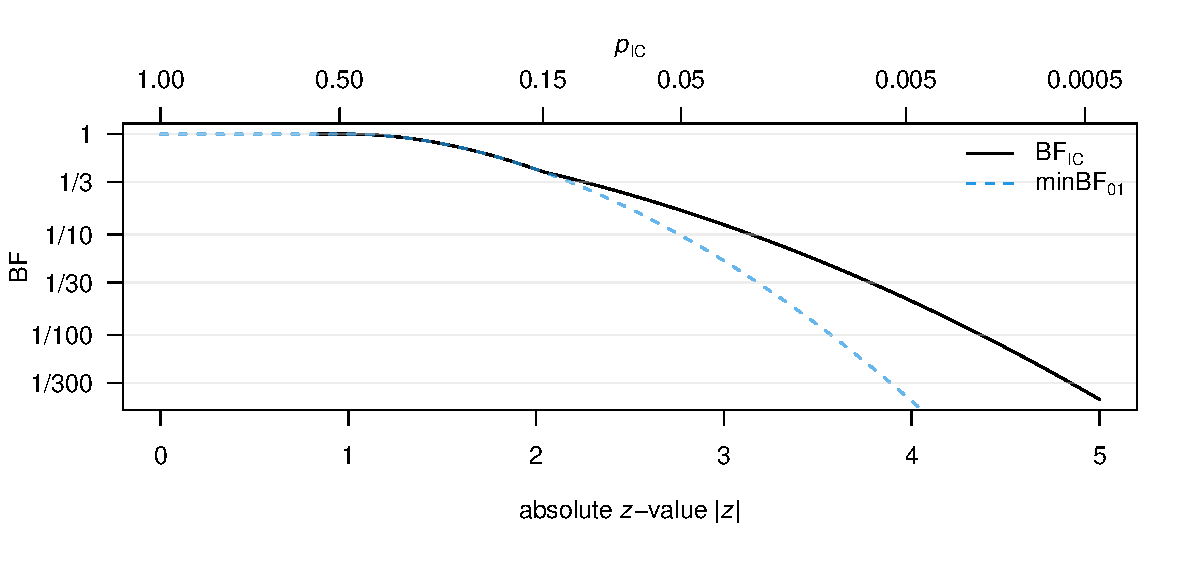
\includegraphics[width=\maxwidth]{images/paper4/example5-RECOVERY-1}
}
\end{knitrout}
\caption{Comparison of the Bayes factor for intrinsic credibility $\BFIC$, the
  minimum Bayes factor $\mbox{minBF}_{01}$, and the $p$-value for intrinsic
  credibility $\pIC$ as a function of the absolute $z$-value $\abs{z}$. The
  value $\pIC = 0.15$ is at the breakpoint at $\abs{z} = 2.04$.}
\label{fig4:bfic}
\end{figure}

The plausibility of the sufficiently sceptical prior can be evaluated in light
of external evidence, but what should we do in the absence of such? We could
again use the \citet{Box1980} prior-predictive check as in
Section~\ref{sec4:IC}, however, the resulting tail probability is difficult to
compare to the Bayes-factor cut-off $\gamma$. When a specific alternative model
to the null is in mind, \citet[p. 391]{Box1980} also suggested to use a Bayes
factor for model criticism of the null model. Following this approach,
\citet{Pawel2020b} proposed to define a second Bayes factor contrasting the
sufficiently sceptical prior to an optimistic prior, which they defined as
\mbox{$\theta \given H_2 \sim \Nor(\hat{\theta}, \sigma^2)$} the posterior of
$\theta$ based on the data and the reference prior $f(\theta) \propto 1$. The
optimistic prior therefore represents the position of a proponent who takes the
original claim at face value. This leads to the second Bayes factor being
\begin{align}
  \label{eq4:bf12}
  \BF_{12} = \sqrt{\frac{2}{1 + g}} \cdot \exp\left\{-\frac{1}{2}\cdot \frac{z^{2}}{1 + g}\right\}.
\end{align}
Analogously to the tail probability approach from Section~\ref{sec4:IC},
intrinsic credibility is established if the data support the optimistic over the
sceptical prior at a higher level than they support the sceptical prior over the
null hypothesis, \ie{} if
\begin{align*}
  \BF_{12} \leq \BF_{01}
\end{align*}
with sufficiently sceptical relative prior variance $g$ from~\eqref{ggamma} used
in both Bayes factors. For example, if we challenge the RECOVERY trial finding
such that the resulting Bayes factor is only $\BF_{01} = 1/10$, we obtain
with~\eqref{eq4:sspv} the sufficiently sceptical relative prior variance
$g = 0.59$ and in turn with~\eqref{eq4:bf12} the Bayes factor $\BF_{12} = 1/64$,
so the finding is intrinsically credible at $\gamma = 1/10$.

To remove the dependence on the choice of the level $\gamma$, one can determine
the smallest level $\gamma$ where intrinsic credibility can be established. This
defines a Bayes factor for intrinsic credibility $\BFIC$ similar to the
definition of the $p$-value for intrinsic credibility $\pIC$
from~\eqref{eq4:pic}. Intrinsic credibility at level $\gamma$ is then equivalent
with $\BFIC \leq \gamma$. Details on the computation of $\BFIC$ are given in
Appendix~\ref{app:BFIC}. For the RECOVERY finding, the Bayes factor for
intrinsic credibility is $\BFIC = 1/25$. This means the data favour the
optimistic prior over any sceptical prior that is capable of rendering the
original result no longer convincing at $\gamma = 1/25$. For comparison the
$p$-value for intrinsic credibility~\eqref{eq4:pic} is $\pIC = 0.009$.


Figure~\ref{fig4:bfic} shows the Bayes factor for intrinsic credibility $\BFIC$
as a function of the $z$-value along with a comparison to the $p$-value for
intrinsic credibility $\pIC$ and the minimum Bayes factor $\mbox{minBF}_{01}$
from~\eqref{eq4:minBFnorm}. We see that the $\BFIC$ is undefined when
$\abs{z} < \sqrt{\log 2} \approx 0.83$. In this case the data are so
unconvincing that any sceptical prior is better supported by the data than the
optimistic prior. For $z$-values between $\sqrt{\log 2} \leq \abs{z} < 2.04$,
the $\BFIC$ equals the minimum Bayes factor $\mbox{minBF}_{01}$, whereas for
larger $z$-values $\abs{z} \geq 2.04$, the $\BFIC$ is always larger (more
conservative) than the $\mbox{minBF}_{01}$. In the absence of any prior
information, it may therefore be a useful evidential summary which formally
takes into account both scepticism and optimism about the observed data.


A $p$-value less than $0.05$ is usually regarded as sufficient evidence against
the null hypothesis, but how much evidence does $p = 0.05$ mean in terms of the
Bayes factor for intrinsic credibility? From Figure~\ref{fig4:bfic}, we see that
the $\BFIC = 1/2.1$ for $\abs{z} = 1.96$, so at most ``worth a bare mention''
according to the classification from \citet{Jeffreys1961}. Thus, also from this
perspective, the conventional $p$-value threshold of 0.05 for the claim of new
discoveries seems too lax in terms of the evidential value that a finding at
this threshold provides. We saw in Section~\ref{sec4:IC} that an ordinary
$p$-value needs to be at least as small as $p \leq 0.0056$ for a finding to be
intrinsically credible in terms of the $p$-value for intrinsic credibility
$\pIC \leq 0.05$. A $p$-value of 0.0056 corresponds to $\abs{z} = 2.77$ where
the Bayes factor for intrinsic credibility is $\BFIC = 1/5.7$, indicating at
least ``substantial'' evidence against the null hypothesis according to
Jeffreys. To achieve intrinsic credibility at the level for strong evidence
($\gamma = 1/10$) the requirements are even more stringent as the $z$-value
needs to be at least $\abs{z} \geq 3.15$ (equivalent to
$\mbox{minBF} \leq 1/27$, $p \leq 0.002$, or $\pIC \leq 0.026$).

\subsection{Advocacy priors}
A natural question is whether we can also define an advocacy prior, a prior
which renders an uncompelling finding compelling, in the AnCred framework with
Bayes factors. In traditional AnCred, advocacy priors always exist since one can
always find a prior that, when combined with the data, can overrule them. This
is fundamentally different to inference based on Bayes factors, where the prior
is not synthesized with the data, but rather used to predict them. A classical
result due to \citet{Edwards1963} states that if we consider the class of all
possible priors under $H_1$, the minimum Bayes factor is given by
\begin{equation}\label{eq4:ELSminBF}
  \text{minBF}_{01} = \exp\left\{-z^2/2\right\}
\end{equation}
which is obtained for $H_1$: $\theta = \hat{\theta}$. This implies that a
non-compelling finding can not be ``rescued'' further than to this bound. For
example, for the finding from the REMAP-CAP trial the bound is unsatisfactorily
$\text{minBF}_{01} = 1/1.7$, so at most ``worth a bare mention'' according to
the classification from \citet{Jeffreys1961}.

Putting these considerations aside, we may still consider the class of
$\Nor(\mu, \tau^2)$ priors under the alternative $H_1$. The Bayes factor
contrasting $H_0$ to $H_1$ is then given by
\begin{align*}
  \BF_{01}
  &= \sqrt{1 + \tau^2/\sigma^2} \cdot \exp\left\{-\frac{1}{2}\left[
  \frac{\hat{\theta}^2}{\sigma^2} - \frac{(\hat{\theta} - \mu)^2}{\sigma^2 +
  \tau^2}\right]\right\}.
\end{align*}
The Reverse-Bayes approach now determines the prior mean $\mu$ and variance
$\tau^2$ which lead to the Bayes factor $\BF_{01}$ being just at some cut-off
$\gamma$. However, if both parameters are free, there are infinitely many
solutions to $\BF_{01} = \gamma$, if any exist at all. The traditional AnCred
framework resolves this by restricting the class of possible priors to advocacy
priors with fixed coefficient of variation of
$\text{CV} = \tau/\mu = 1/z_{\alpha/2}$. We can translate this idea to the Bayes
factor AnCred framework and fix the prior's coefficient of variation to
$\text{CV} = 1/z(\gamma)$, where
\begin{align}
  z(\gamma) = \sqrt{- 2 \, \log \gamma}, \label{eq4:zgamma}
\end{align}
obtained by solving \eqref{eq4:ELSminBF} for $z$ with
$\text{minBF}_{01} = \gamma$. The advocacy prior thus carries the same
evidential weight as data with $\text{minBF}_{01} = \gamma$. Moreover, the
determination of the prior parameters becomes more feasible since there is only
one free parameter left (either $\mu$ or $\tau^2$).


The right plot in Figure \ref{fig4:bf} illustrates application of the procedure
on data from the meta-analysis on association between COVID-19 mortality and
corticosteroids. The coefficient of variation of the advocacy prior is fixed to
$\text{CV} = 1/z(\gamma=1/3) = 0.67$ (for comparison, the CV of the advocacy
prior in traditional AnCred at $\alpha = 0.05$ is
$\text{CV} = 1/z_{\alpha/2}= 0.51$) and thus the Bayes factor $\BF_{01}$ only
depends on the relative mean $f = \mu/\hat{\theta}$. Under the sceptical prior
only the RECOVERY finding could be challenged at $\gamma = 1/3$ (where
$z(\gamma)=1.5$ corresponds to $\alpha=13$\%). With the advocacy prior this is
now also possible for the CAPE COVID finding \citep{Dequin2020}, where a prior
with mean $\mu = f \cdot \hat{\theta} = 0.37 \cdot (-0.79) = -0.29$ and standard
deviation $\tau = \text{CV} \cdot \mu = 0.2$ is able to make the finding
compelling at $\gamma = 1/3$. The corresponding prior credible interval for the
OR at level $1-\alpha$ ranges from 0.55 to 1, so advocates may still consider
the ``non-compelling'' finding as providing moderate evidence in favour of a
benefit, if external evidence supports mortality reductions in that range. Using
the prior-to-data conversion described in
Section~\ref{sec4:prior-data-translation}, the prior can be translated to a
trial with 69 events in both arms, but 206 non-events in the treatment and 182
non-events in the control arm (such that the mortality rate in the control arm
is the same as in the CAPE COVID trial). Note that the advocacy prior may not be
unique, \eg{} for the CAPE COVID finding the prior with relative mean
$f^\prime = 1.26$ and standard deviation $\tau^\prime = 0.67$ also renders the
data as just compelling at $\gamma = 1/3$. We recommend to choose the prior with
$f$ closer to zero, as it is the more conservative choice.

\section{Reverse-Bayes analysis of the False Positive Risk}
\label{sec4:p.equals}

Application of the Analysis of Credibility with Bayes factors as described in
Section \ref{sec4:bfs} assumes some familiarity with Bayes factors as measures
of evidence. \citet{Colquhoun2019} argued that very few nonprofessional users of
statistics are familiar with the notion of Bayes factors or likelihood ratios.
He proposes to quantify evidence with the \emph{false positive risk}, ``if only
because that is what most users still think, mistakenly, that that is what the
$p$-value tells them''. More specifically, \citet{Colquhoun2019} defines the
\FPR{} as the posterior probability that the point null hypothesis $H_0$ of no
effect is true given the observed $p$-value $p$, \ie{} $\FPR = \Pr(H_0 \given p)$.
As before, $H_0$ corresponds to the point null hypothesis $H_0\colon$
$\theta = 0$. Note also that we take the exact (two-sided) $p$-value $p$ as the
observed ``data'', regardless of whether or not it is significant at some
pre-specified level, the so-called ``$p$-equals'' interpretation of NHST
\citep{Colquhoun2017}.


$\FPR$ can be calculated based on the Bayes factor associated with $p$. For ease
of presentation we invert Bayes' theorem \eqref{eq4:eq0} and obtain
\begin{equation}\label{eq4:bayes}
      \frac{\FPR}{1-\FPR} = \frac{\Pr(H_0 \given p)}{\Pr(H_1 \given p)}
      = {\mbox{BF}_{01}} \, \frac{\Pr(H_0)}{\Pr(H_1)},
\end{equation}
where $\mbox{BF}_{01}=1/\mbox{BF}_{10}$ is the Bayes factor for $H_0$ against
$H_1$, computed directly from the observed $p$-value $p$.

The common 'forward-Bayes' approach is to compute the $\FPR$ from the prior
probability $\Pr(H_0)$ and the Bayes factor with \eqref{eq4:bayes}. However, the
prior probability $\Pr(H_0)$ is usually unknown in practice and often hard to
assess. This can be resolved via the Reverse-Bayes approach
\citep{Colquhoun2017,Colquhoun2019}: Given a $p$-value and a false positive risk
value, calculate the corresponding prior probability $\Pr(H_0)$ that is needed
to achieve that false positive risk. Of specific interest is the value FPR =
5\%, because many scientists believe that a Type I error of 5\% is equivalent to
a FPR of 5\% \citep{Greenland2016}. This is of course not true and we follow
Example 1 from \citet{Berger1987} and use the Reverse-Bayes approach to derive
the necessary prior assumptions on $\Pr(H_0)$ to achieve FPR = 5\% with Equation
\eqref{eq4:bayes}:
\begin{equation}
  \label{eq4:prior.prob}
     \Pr(H_0) = \left[ 1 + \frac{1-\FPR}{\FPR} \cdot \mbox{BF}_{01}  \right]^{-1}.
\end{equation}

\citet{Colquhoun2017} uses a Bayes factor based on the $t$-test, but for
compatibility with the previous sections we assume normality of the underlying
test statistic. We consider Bayes factors under all simple alternatives, but
also Bayes factors under local normal priors, see \citet{Held2018} for a
detailed comparison.

Instead of working with a Bayes factor for a specific prior distribution, we
prefer to work with the minimum Bayes factor $\mbox{minBF}_{01}$ as introduced
in Section \ref{sec4:sceptical}. In what follows we will use the minimum Bayes
factor based on the $z$-test, see Section 2.1 and 2.2 in \citet{Held2018}.


Let $\mbox{minBF}_{01}$ denote the minimum Bayes factor over a specific class of
alternatives. From equation \eqref{eq4:prior.prob} we obtain the inequality
\begin{equation}\label{eq4:prior.prob2}
    \Pr(H_0) \leq \left[ 1 + \frac{1-\FPR}{\FPR} \cdot \mbox{minBF}_{01}  \right]^{-1}.
\end{equation}
The right-hand side is thus an upper bound on the prior probability $\Pr(H_0)$
for a given $p$-value to achieve a pre-specified FPR value.


There are also minBFs not based on the $z$-test statistic
as~\eqref{eq4:minBFnorm}, but directly on the (two-sided) $p$-value $p$, the
so-called ``$- e \, p \log p$'' \citep{Sellke2001} calibration
\begin{equation}
\label{eq4:sbb}
{\mbox{minBF}} =  \left\{ \begin{array}{ll} - e \, p \log p & \mbox{ for } p < 1/e \\
  1 & \mbox{ otherwise, } \end{array}   \right.
\end{equation}
and the ``$- e \, q \log q$'' calibration, where $q = 1-p$, see Section 2.3 in
\citet{Held2018}:
\begin{equation}
\label{eq4:sbb2}
{\mbox{minBF}} =  \left\{ \begin{array}{ll} - e \, (1-p) \log (1-p) & \mbox{ for } p < 1-1/e \\
  1 & \mbox{ otherwise. } \end{array}   \right.
\end{equation}
For small $p$, equation \eqref{eq4:sbb2} can be simplified to
${\mbox{minBF}} \approx e \, p$, which mimics the \citet{Good1958}
transformation of $p$-values to Bayes factors \citep{Held2019b}.

The two $p$-based calibrations carry less assumptions than the minimum Bayes
factors based on the $z$-test under normality and can be used as alternative
expressions in~\eqref{eq4:prior.prob2}. The ``$- e \, p \log p$'' provides a
general bound under all unimodal and symmetrical local priors for $p$-values
from $z$-tests, see Section 3.2 in \citet{Sellke2001}. The ``$- e \, q \log q$''
calibration is more conservative and gives a smaller bound on the Bayes factor
than the ``$- e \, p \log p$'' calibration. It can be viewed as a general lower
bound under simple alternatives where the direction of the effect is taken into
account, see Section 2.1 and 2.3 in \citet{Held2018}.

\begin{figure}[!htb]
\begin{knitrout}
\definecolor{shadecolor}{rgb}{0.969, 0.969, 0.969}\color{fgcolor}
{\centering 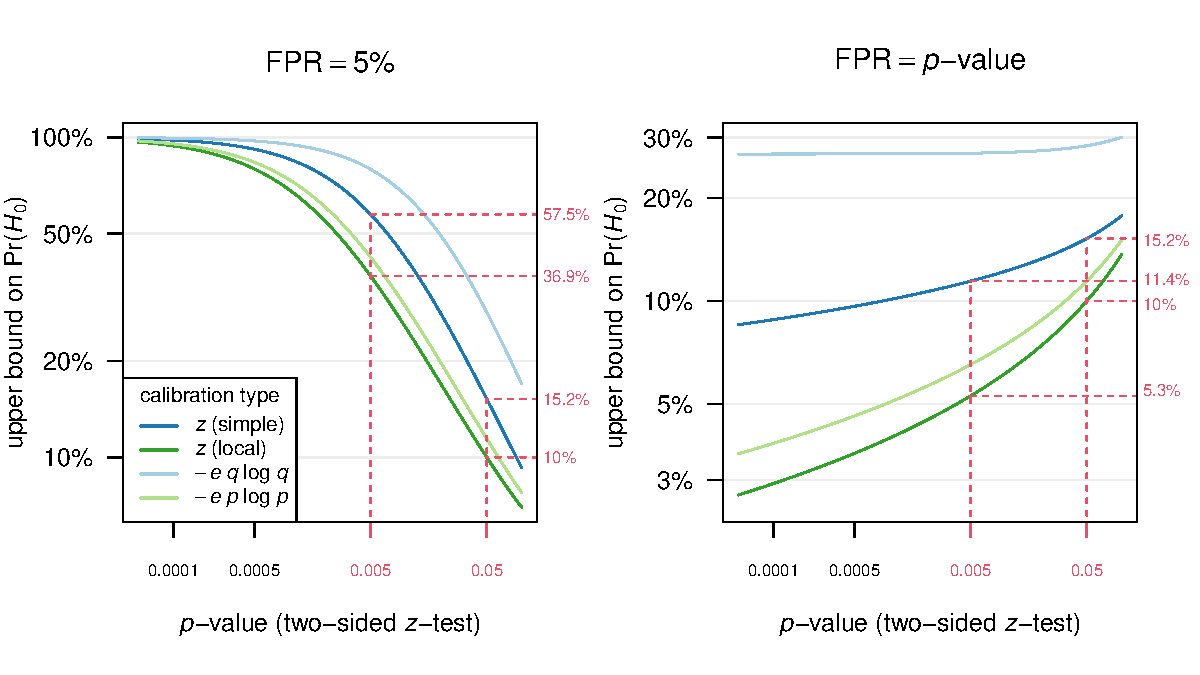
\includegraphics[width=\maxwidth]{images/paper4/FPR-plot-1}
}
\end{knitrout}
\caption{The left plot shows the upper bound on the prior probability $\Pr(H_0)$
  to achieve a false positive risk of 5\% as a function of the $p$-value
  calibrated with either a $z$-test calibration (simple or local alternatives)
  or with the ``$- e \, p \log p$'' or ``$- e \, q \log q$'' calibrations,
  respectively. The right plot shows the upper bound on $\Pr(H_0)$ as a function
  of the $p$-value using the same calibrations but assuming the $p$-value equals
  the $\FPR$.}
\label{fig4:fpr}
\end{figure}

The left plot in Figure \ref{fig4:fpr} shows the resulting upper bound on the
prior probability $\Pr(H_0)$ as a function of the two-sided $p$-value if the FPR
is fixed at 5\%. For $p=0.05$, the ``$- e \, p \log p$'' bound is around 11\%
and 28\% for the ``$- e \, q \log q$'' calibration. The corresponding values
based on the $z$-test are slightly smaller (10\% and 15\%, respectively). All
the probabilities are below the 50\% value of equipoise, illustrating that
borderline significant result with $p \approx 0.05$ do not provide sufficient
evidence to justify an FPR value of 5\%. For $p=0.005$, the upper bounds are
closer to 50\% (37\% for local and 57\% for simple alternatives).


Turning again to the example from the RECOVERY trial, the $p$-value associated
with the estimated treatment effect is $p = 0.0002$. The left plot in Figure
\ref{fig4:fpr} shows that the false positive risk can safely be assumed to be
around 5\% (or lower), since the upper bound on $\Pr(H_0)$ are all very large
for such a small $p$-value.

Fixing FPR at the 5\% level may be considered as arbitrary. Another widespread
misconception is the belief that the FPR is equal to the $p$-value.
\citet{Held2013} used a Reverse-Bayes approach to investigate which prior
assumptions are required such that $\FPR=p$ holds. Combining
\eqref{eq4:prior.prob} with the ``$- e \, p \log p$'' calibration
\eqref{eq4:sbb} gives the explicit condition
\begin{equation*}
  \Pr(H_0) \leq 1/\left\{ 1 - e \, (1-p) \, \log(p) \right\}
\end{equation*}
whereas the ``$- e \, q \log q$'' calibration \eqref{eq4:sbb2} leads to
\begin{equation*}
  \Pr(H_0) \leq 1/\left\{ 1 - e \, \frac{(1-p)^2}{p} \, \log(1-p) \right\} \approx 1/\left\{ 1 + e \, (1-p) \right\},
\end{equation*}
which is approximately $1/(1+e)=26.9$\% for small $p$.

The right plot in Figure \ref{fig4:fpr} compares the bounds based on these two
calibrations with the ones obtained from simple respectively local alternatives.
We can see that strong assumptions on $\Pr(H_0)$ are needed to justify the claim
$\FPR=p$: $\Pr(H_0)$ cannot be larger than 15.2\% if the $p$-value is
conventionally significant ($p<0.05$). For $p<0.005$, the bound drops further to
11.4\%. Even under the conservative ``$- e \, q \log q$'' calibration, the upper
bound on $\Pr(H_0)$ is $26.9$\% for small $p$ and increases only slightly for
larger values of $p$. This illustrates that the misinterpretation $\FPR=p$ only
holds if the prior probability of $H_0$ is substantially smaller than 50\%, an
assumption which is questionable in the absence of strong external knowledge.

\section{Discussion}

\subsection{Extensions, work in progress and outlook}
\label{sec4:extensions}
The Reverse-Bayes methods described above have focused on the comparison of the
prior needed for credibility with findings from other studies and/or more
general insights. However, replication studies make an obvious additional source
of external evidence, as these are typically conducted to confirm original
findings by repeating their experiments as closely as possible. The question is
then whether the original findings have been successfully ``replicated'',
currently of considerable concern to the research community. To date, there
remains no consensus on the precise meaning of replication in a statistical
sense. The proposal of \citet{Held2020} \citep[see also][]{Held2021} was to
challenge the original finding using AnCred, as described in Section
\ref{sec4:AnCred}, and then evaluate the plausibility of the resulting prior
using a prior-predictive check on the data from a replication study. A similar
procedure but using AnCred based on Bayes factors as in Section \ref{sec4:bfs}
was proposed in \citet{Pawel2020b}. Reverse-Bayes inference seems to fit
naturally into this setting as it provides a formal framework to challenge and
substantiate scientific findings.


Apart from using data from a replication study, there are also other possible
extensions of AnCred: We proposed to derive Reverse-Bayes priors using posterior
tail probabilities (or credible intervals) or Bayes factors as measures of
evidence, but also other measures such as relative belief ratios
\citep{Evans2015} could be used. When testing point null hypotheses, relative
belief ratios are equivalent to Bayes factors due to the Savage-Dickey density
ratio \citep[p. 98]{Evans2015}. Therefore, determining the sceptical prior
variance through fixing the resulting Bayes factor is equivalent to fixing the
resulting relative belief ratio. However, there is no connection to relative
belief in prior-data conflict assessment based on the Bayes factor contrasting
the sceptical to the optimistic prior since both are composite. Further research
is needed on Reverse-Bayes procedures in the relative belief framework,
candidate methods for prior-data conflict assessment are prior to posterior
divergence \citep{Nott2020} and prior expansions \citep{Nott2021} as these
methods have an interpretation in terms of relative beliefs. Moreover, we either
used prior-predictive checks \citep{Box1980, Evans2006} or Bayes-factors
\citep{Jeffreys1961, Kass1995} for the formal evaluation of the plausibility of
the priors derived through Reverse-Bayes. Other methods could be used for this
purpose, for example, Bayesian measures of surprise \citep{Bayarri2003}.
Furthermore, AnCred in its current state is derived assuming a normal likelihood
for the effect estimate $\hat{\theta}$. This is the same framework as in
standard meta-analysis and provides a good approximation for studies with
reasonable sample size \citep{Carlin1992}. For the comparison of binomial
outcomes with small counts, the normal approximation of the log odds ratio could
be improved with a Yates continuity correction \citep[section
2.4.1]{Spiegelhalter2004} or replaced with the exact profile likelihood of the
log odds ratio \citep[section 5.3]{Held2014}, see also Section 4 in
\citet{Pawel2020b} which shows AnCred with Bayes factors using either a
non-central $t$ or a Binomial likelihood. Likewise, the conjugate normal prior
could be replaced by a more robust prior distribution such as a mixture of
normals (as considered in Section~\ref{sec4:nonSigAnCred}), a
double-exponential, or a Student $t$-distribution \citep{Pericchi1992}. For
example, \citet{Fuquene2009} investigate the use of robust priors in an
application to binomial data from a randomized controlled trial. In general, any
distribution from the location-scale family can be used, whereby the scale
parameter takes over the role of the sceptical prior standard deviation, while
the location parameter is fixed to the null value.

\subsection{Conclusions}
The inferential advantages of Bayesian methods are increasingly recognised
within the statistical community. However, among the majority of working
researchers they have failed to make any serious headway, and retain a
reputation for complex and ``controversial''. We have outlined how an idea that
began with Jack Good's proposal for resolving the ``Problem of Priors'' over 70
years ago \citep{Good1950} has experienced a renaissance over recent years. The
basic idea is to invert Bayes' theorem: a specified posterior is combined with
the data to obtain the Reverse-Bayes prior, which is then used for further
inference. This approach is useful in situations where it is difficult to decide
what constitutes a reasonable prior, but easy to specify the posterior which
would lead to a particular decision. A subsequent prior-to-data conversion
\citep{Greenland2006} helps to assess the weight of the Reverse-Bayes prior in
relation to the actual data.

We have shown that the Reverse-Bayes methodology is useful to extract more
insights from the results typically reported in a meta-analysis. It facilitates
the computation of prior-predictive checks for conflict diagnostics
\citep{Presanis2013} and has been shown capable of addressing many common
inferential challenges, including assessing the credibility of scientific
findings \citep{Spiegelhalter2004,Greenland2011}, making sense of ``out of the
blue'' discoveries with no prior support \citep{Matthews2018, Held2019a},
estimating the probability of successful replications \citep{Held2019a,
  Held2020}, and extracting more insight from standard $p$-values while reducing
the risk of misinterpretation \citep{Held2013,Colquhoun2017,Colquhoun2019}. The
appeal of Reverse-Bayes techniques has recently been widened by the development
of inferential methods using both posterior probabilities and Bayes Factors
\citep{Carlin1996, Pawel2020b}.

These developments come at a crucial time for the role of statistical methods in
research. Despite the many serious -- and now well-publicised – inadequacies of
NHST \citep{Wasserstein2016}, the research community has shown itself to be
remarkably reluctant to abandon NHST. Techniques based on the Reverse-Bayes
methodology of the kind described in this review could encourage the wider use
of Bayesian inference by researchers. As such, we believe they can play a key
role in the scientific enterprise of the 21\textsuperscript{th} century.



\section*{Software and Data Availability}
All analyses were performed in the R programming language version 4.2.2
\citep{R}. Minimum Bayes factors were computed using the package
\texttt{pCalibrate} \citep{Held2018}. The package \texttt{metafor}
\citep{Viechtbauer2010} was used for meta-analysis and forest plots. Data and
code to reproduce all analyses are available at
\url{https://gitlab.uzh.ch/samuel.pawel/Reverse-Bayes-Code}.

\section*{Acknowledgments}
We are grateful to Sander Greenland for helpful comments on a previous version
of this article. We also acknowledge detailed comments by an Associate Editor
and two referees, that helped to improve the manuscript.


\begin{subappendices}
\renewcommand{\thesection}{\Alph{section}}
\section{Mean of the advocacy prior}
\label{app:app1}
Suppose that the estimate $\hat \theta$ is not significant at level $\alpha$, so
$z^2/z_{\alpha/2}^2<1$. With $U,L = \hat \theta \pm z_{\alpha/2} \, \sigma$ we
have $U + L = 2 \, \hat \theta$,
$U L = \hat \theta^2 - z_{\alpha/2}^2 \, \sigma^2$ and $U-L =
2 \, z_{\alpha/2} \, \sigma$.

We therefore obtain with \eqref{eq4:AL}:
\begin{equation*}
\mu = \frac{\mbox{AL}}{2} =  - \frac{2 \, \hat \theta}{2 \, (\hat \theta^2 - z_{\alpha/2}^2 \, \sigma^2)} \frac{(2 \, z_{\alpha/2} \, \sigma)^2}{2}
 =  \frac{2 \, \hat \theta \, z_{\alpha/2}^2 \, \sigma^2}{z_{\alpha/2}^2 \, \sigma^2 - \hat \theta^2}
 =  \frac{2 \, \hat \theta}{1 - z^2/z_{\alpha/2}^2}.
\end{equation*}
Dividing by the effect estimate $\hat{\theta}$ leads to the relative mean
$f = \mu/\hat{\theta}$ as in~\eqref{eq4:mu}. The advocacy standard deviation is
$\tau = {\mbox{AL}}/{(2 \, z_{\alpha/2})} = {\mu}/{z_{\alpha/2}}$ and the
coefficient of variation is therefore
$\mbox{CV} = \tau/\mu = z_{\alpha/2}^{-1}$.

\section{Bayes factor for intrinsic credibility}
\label{app:BFIC}
Intrinsic credibility at level $\gamma$ is established when
\begin{align}
  \label{eq4:ic-condition}
  \BF_{12} \leq \BF_{01} = \gamma
\end{align}
and we are interested in the Bayes factor for intrinsic credibility $\BFIC$
which is the smallest level $\gamma \in (0, 1]$ where~\eqref{eq4:ic-condition}
holds. The $\BFIC$ is therefore a special case of the sceptical Bayes factor
from \citet{Pawel2020b} where the same data is used in both Bayes factors
(instead of the data from a replication study for $\BF_{12}$). It is hence given
by
\begin{align}
  \label{eq4:BFic}
  \BFIC =
  \begin{cases}
    \sqrt{-z^{2}/k}\cdot \exp\left\{-(z^{2} + k)/2\right\}
    & \text{if} \abs{z} \geq \surd\big\{-2 \mathrm{W}\big(-e^{-1}/\sqrt2\big)\big\}\\
    \mbox{minBF}_{01} \
    & \text{if} ~ \sqrt{\log 2} \leq \abs{z} < \surd\big\{-2 \mathrm{W}\big(-e^{-1}/\sqrt2\big)\big\} \\
    \text{undefined}
    & \text{if} ~ \abs{z} < \sqrt{\log 2}
  \end{cases}
\end{align}
with $k = \mathrm{W}(-z^{2} \exp\{-z^{2}/2\}/\sqrt{2})$ and $\mathrm{W}(\cdot)$
the branch of the Lambert W function that satisfies $\mathrm{W}(y) \leq -1$ for
$y \in [-e^{-1}, 0).$ If
$\abs{z} \geq \sqrt{-2 \mathrm{W}(-e^{-1}/\sqrt2)} \approx 2.04$, $\BFIC$ is
located at the intersection between $\BF_{12}$ and $\BF_{01}$ in the relative
prior variance $g$, so equation (7) from \citet{Pawel2020b} can be used. For
$\abs{z} \geq \sqrt{\log 2} \approx 0.83$, $\BF_{12}$ remains below $\BF_{01}$
for all $g$ and hence $\BFIC$ is given by $\mbox{minBF}_{01}$, the minimum of
$\BF_{01}$ from \eqref{eq4:minBFnorm}. Finally, when $\abs{z} < \sqrt{\log 2}$,
equation~\eqref{eq4:ic-condition} cannot be satisfied for any valid sufficiently
sceptical relative prior variance $g$, hence the $\BFIC$ is undefined.

\end{subappendices}

\bibliographystyle{apalikedoiurl}
\bibliography{bibliography}
